\chapter{Presenting Your Venture}

Joseph Hadzima frames this evening as a paired lesson: first we learn how to present the venture, and then we learn how to negotiate around it. Bob Jones takes the first half and argues that presenting is not decoration. A venture must be explained to customers, recruits, partners, investors, and sometimes even to skeptical family members. These notes follow the MIT OpenCourseWare session framed by Hadzima and delivered by Jones, with the present volume curated by LazyingArt LLC. We shall therefore treat the pitch as a structured object: a map from problem to audience-specific benefit, and from benefit to the action we want the listener to take.

\section{Why Presenting a Venture Belongs in the Course}

Jones does not begin with technique. He begins by asking why a course on venture formation should spend scarce time on presentation at all. The answer he draws from the room is value creation, and he immediately makes that answer concrete. It is hard to raise money without talking to investors; hard to acquire customers without talking to customers; hard to recruit talent without convincing people to join a risky enterprise.

Before we ever reach a formal theory of the pitch, Jones inserts a useful business ladder. He reminds us that the entrepreneurial chain contains several distinct transformations:
\begin{equation}
\text{Idea} \neq \text{Product}, \qquad \text{Product} \neq \text{Business}.
\end{equation}
A good idea does not yet answer questions of packaging, pricing, execution, or market fit. A good product does not yet amount to a good business. And a good business must still be describable. One of Jones's tests is brutally simple: if someone asks us about our company and, half an hour later, we are still struggling for words, that is already evidence that we do not understand the business as well as we think we do.

This opening matters for the whole lecture. Presentation is not treated as polish added at the end. It is treated as evidence of whether the entrepreneur understands the thing being built.

\section{Audiences, Objectives, and the Meaning of a Pitch}

Jones next narrows the subject. A pitch is not just speech. It is speech with a target.

\begin{definition}
A pitch is a presentation oriented toward a specific audience \(A\), aimed at producing a desired behavior \(Y\), shaped by what that audience wants \(W_A\), and ending in the speaker's ask \(G\).
\end{definition}

We may compress this into a simple schema:
\begin{equation}
\text{Pitch}=(A,\ Y,\ W_A,\ G).
\end{equation}
This is not Jones's notation, but it is faithful to the questions he explicitly asks: to whom are we speaking, why are we speaking to them, what do they want, how do we give them what they want, and what do we want from them?

At this point the lecture moves from general importance to the first audience list. The available visual evidence records that transition in a partial, still-unfolding state.

\begin{figure}[h]
\centering

\includegraphics[width=\linewidth]{lecture_06_figure_02.png}
\caption{Early audience list for a venture pitch: customers and potential employees. The frame captures a partial reveal state, not the complete list discussed later in the lecture.}
\end{figure}

\begin{remark}
The validated frame shows only \textit{Customers} and \textit{Potential employees}. The transcript later extends the list to current employees, channel partners or retailers, family members, and investors. We should not read those later items back into the image itself.
\end{remark}

Even in this partial form, the slide does important work. It marks the shift from a generic notion of “communication” to the harder problem of audience selection. Jones is building a taxonomy one step at a time.

In the fuller spoken list, the relevant audiences are approximately
\[
A_{\text{full}}=\{\text{customers},\ \text{potential employees},\ \text{current employees},\ \text{channel partners / retailers},\ \text{family members},\ \text{investors}\}.
\]

\subsection{Question \& Answer}

\paragraph{Question.} Should every audience get the same pitch?

\paragraph{Answer.} No. Jones asks this directly and answers it directly. Different audiences do not share the same priorities, so there is no reason to expect that the same framing, the same benefits, or the same level of detail will work for all of them. The entrepreneur who is recruiting an engineer is not solving the same problem as the entrepreneur who is asking an investor for capital, and neither is solving the same problem as the entrepreneur who is trying to win a customer.

\section{The Audience's Hidden Question: WIFM}

The lecture's first strong compression arrives here. Jones introduces a sales acronym, but the point is broader than sales. Every audience is silently running the same filter:
\begin{equation}
\mathrm{WIFM}(A)=\text{``What's in it for me?''}
\end{equation}
The listener may be too polite or too sophisticated to say this out loud, but the question is present all the same. A successful pitch answers it before the audience has to ask.

For a customer, the translation is immediate. The customer is not mainly interested in the founder's brilliance or the elegance of the technology. The customer wants the relevant problem solved. Jones gives simple illustrations: can the app get me where I want to go, quickly and efficiently? does this purchase help me appear as I need to appear? In each case, the audience evaluates the pitch through its own desired outcome.

For a potential employee, the hidden question changes. The recruit may think the technology is interesting, but that is not the main issue. Can I pay my bills? Am I joining something stable enough to survive? Will I matter here, or am I merely being asked to admire the founder's invention? The same venture therefore has to be translated into a different benefit language.

A compact transcript-derived diagram is helpful here:

\begin{figure}[h]
\centering
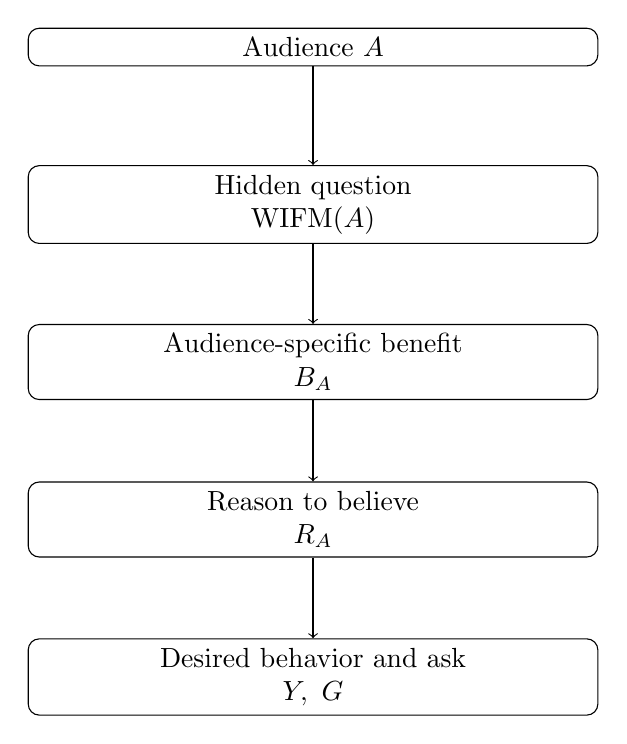
\begin{tikzpicture}
\node[draw, rounded corners, align=center, text width=7cm] (a) at (0,0) {Audience \(A\)};
\node[draw, rounded corners, align=center, text width=7cm] (b) at (0,-2.0) {Hidden question\\\(\mathrm{WIFM}(A)\)};
\node[draw, rounded corners, align=center, text width=7cm] (c) at (0,-4.0) {Audience-specific benefit\\\(B_A\)};
\node[draw, rounded corners, align=center, text width=7cm] (d) at (0,-6.0) {Reason to believe\\\(R_A\)};
\node[draw, rounded corners, align=center, text width=7cm] (e) at (0,-8.0) {Desired behavior and ask\\\(Y,\ G\)};
\draw[->] (a) -- (b);
\draw[->] (b) -- (c);
\draw[->] (c) -- (d);
\draw[->] (d) -- (e);
\end{tikzpicture}
\caption{Transcript-derived pitch logic in narrow form. The pitch is audience-conditioned from the first step.}
\end{figure}

We may therefore summarize the structure of the lecture so far in a single line:
\begin{equation}
A \longrightarrow \mathrm{WIFM}(A) \longrightarrow B_A.
\end{equation}
Only after that do we earn the right to discuss proof, traction, or technical details.

\section{Baseline Pitches and What They Reveal}

Jones then changes tempo. Rather than continuing with abstract instruction, he establishes a baseline by inviting volunteers to pitch. The pedagogical move is important: the lecture now becomes diagnostic.

The first volunteer intends to pitch prospective engineers, but the pitch is dominated by technical difficulty and the size of the video market. This is not useless information, but it is the wrong opening for the chosen audience. The audience has been told it is being recruited, yet it hears almost nothing about the work, the role, the growth path, or the reasons to join. The class's critique is sharp and correct. A recruiting pitch that does not make the job visible has missed the audience.

Jones then supplies a short rewrite. He keeps the unmet need in video editing, introduces the technology only insofar as it matters, and moves quickly to the real appeal: engineers who want to matter, who do not want to vanish into a giant corporation, and who want to come somewhere they can make a difference. The point is not that his exact wording is canonical. The point is that he has translated the venture into the recruit's benefit language.

The second volunteer pitches a medical-imaging venture to investors. Here the failure is different. The opening wanders, the payer is unclear, the market is unclear, and the speaker does not yet show why the investor should believe the venture can get from problem to business. Again Jones intervenes, this time with a fictitious but structurally cleaner rewrite. He begins with the high-risk patient group, moves to telehealth as an imperfect current solution, then states the venture's technological improvement, and only then reaches reimbursement, rollout, and business-model validation.

\subsection{Question \& Answer}

\paragraph{Question.} What went wrong when the pitch did not match the audience?

\paragraph{Answer.} In both volunteer cases, the speaker made the audience do the translation work. In the first case, engineers were given technology without a role. In the second, investors were given an overlong medical story before the business logic appeared. The pitch fails whenever the benefit, the payer, the ask, or the next action must be inferred by the listener rather than supplied by the speaker.

\section{Benefits First, Then Reason to Believe}

Having used the live examples to expose failure modes, Jones now states the central rule of the lecture. We may write it compactly as
\begin{equation}
\text{Problem} \longrightarrow B_A \longrightarrow R_A \longrightarrow G.
\end{equation}
First the problem, then the audience-specific benefit, then the reason to believe, and only then the ask.

This is the meaning of his repeated phrase: benefits first, reason to believe second. If we reverse the order, we force the listener to infer the benefit from the machinery. Jones insists that this is a mistake.

He gives several examples. The cell-phone example is deliberately simple. If we begin by saying that we possess some remarkable technology, the audience has to decide whether to care. If instead we begin with the benefit---instant recharge at the moment the battery is dying---interest arrives before technical explanation. Only afterward do we need to justify belief.

The da Vinci letter drives the point home historically. Jones retells Leonardo not as a painter introducing his artistic genius, but as an engineer promising what the Duke most wants: bridges, siege devices, armored wagons, ways to damage the enemy and defend a city. The Duke is not first captivated by technology in the abstract. He is captivated by benefits stated in his own language.

The Nordstrom anecdote makes the same point in a commercial rather than military register. The salesman begins not with cloth quality or buttonholes, but with the customer's use case. What sort of work do you do? What kind of suit do you need? Only after the desire is established does the supporting evidence matter. The suit is wanted because it solves the appearance problem; the construction details merely justify the purchase already underway.

A useful way to formalize Jones's rule is this:
\begin{align}
B_A &= \text{the payoff the audience cares about},\\
R_A &= \text{the evidence that this payoff can actually be delivered}.
\end{align}
The entrepreneur is often tempted to start with \(R_A\): patents, algorithms, founders, visionary claims. Jones's point is that \(R_A\) has force only after the audience knows why it should care.

\section{Delivery Under Constraints: Time, Memory, Voice, and Practice}

The lecture next shifts from content to constraint. Even a well-structured pitch can fail if it cannot be heard, processed, or remembered. Jones treats this not as a cosmetic problem but as a competitive one.

The memory side of the constraint can be summarized by a small set of lecture heuristics:
\begin{align}
N_{\text{remembered}} &\approx 3,\\
N_{\text{sentences}} &= 3,\\
t_{\text{value prop}} &\approx 10\,\text{s},\\
d_{\text{mic}} &\approx 2\text{--}4\,\text{in}.
\end{align}
Most listeners retain only a few things. Therefore we must decide in advance what those few things are. Jones turns this into a practical challenge: give the value proposition in three sentences and about ten seconds. Hard as that is, it becomes a north star. If we cannot compress the venture that far, the pitch will drift.

The physical side of the constraint is equally concrete. Jones tells a story about winning a pitch contest not because his deck was intrinsically superior, but because he was the only speaker the judges could understand. This leads to the microphone lesson. The microphone is directional; one speaks down the barrel, not over the top, and not from half a foot away. If we point with the same hand that holds the microphone, or if we speed up because our editing was bad, intelligibility collapses.

There is also a pacing constraint. If six minutes of material are squeezed into four minutes by speaking faster, the audience loses the thread. Jones's advice is merciless but correct: edit first, slow down second, and practice until the timing is honest. Practice is not external to the pitch. It is part of the construction of the pitch.

\section{Investor Logic and the Economics of Proof}

When Jones finally narrows the lecture to venture capital, he does so only after establishing the more general framework. That order matters. Investors are not the only audience, but they are one audience whose incentives are particularly easy to formalize.

\subsection{Question \& Answer}

\paragraph{Question.} What do investors actually want to know?

\paragraph{Answer.} Jones reduces the investor's logic to two questions:
\begin{align}
Q_{\text{inv}}^{(1)} &= \text{How will you make money?},\\
Q_{\text{inv}}^{(2)} &= \text{How will I make money?}
\end{align}
Everything else is subordinate. Market, customers, team, manufacturing, sales, and IP all sit under \(Q_{\text{inv}}^{(1)}\). Terms, ownership, exit, and return sit under \(Q_{\text{inv}}^{(2)}\).

Before the pitch even begins, there is an access screen. A pure cold call is said to be almost worthless:
\begin{equation}
N_{\text{cold calls/week}} \approx 200.
\end{equation}
The more promising path is a warm introduction, but that merely adds another filter. The referrer must believe there is audience fit, and must also believe we will not make the referrer look foolish.

Jones is careful here. A short investor pitch is not supposed to complete diligence. Its job is to get the next meeting. It aims at the response, “Yes, I would like to hear more.”

\paragraph{Worked example.} The strongest explicit business arithmetic in the lecture comes not from a student's pitch but from Jones's catheter-lab story. The story begins with a device that doctors and patients like. That is not yet enough, because neither doctors nor patients are the party paying for adoption. Jones therefore changes the audience. He goes to the purchasing department and reframes the value in the hospital's own terms.

The derivation is short:
\begin{enumerate}
\item The cath lab is a revenue-generating part of the hospital.
\item Revenue rises with the number of procedures completed.
\item Turnover lag between procedures is a bottleneck.
\item The device reduces that lag.
\item Therefore throughput rises by one procedure per day.
\item Therefore the device pays for itself quickly.
\end{enumerate}
Jones's own quantitative summary is:
\begin{align}
\Delta n_{\text{procedures/day}} &= 1,\\
T_{\text{payback}} &\approx 6\,\text{weeks}.
\end{align}
He does not show the full arithmetic on the board, and we should not invent it. But the economic structure is clear. Proof of value is not “the doctors liked it.” Proof of value is “the hospital can do one more revenue-producing procedure per day, so the purchase has a short payback period.”

This is the investor lesson as well. The pitch becomes compelling when benefit and proof are aligned with the incentives of the party making the decision.

\subsection{Question \& Answer}

\paragraph{Question.} Who should give the pitch?

\paragraph{Answer.} Jones's answer is nuanced but firm. A team presentation may be best, since a chief technology officer may explain the technical side better and a chief marketing officer may explain go-to-market better. But he says he has never seen an investor commit without confidence that the chief executive can drive the bus. So the presentation may be distributed, but the founder or CEO is not excused from the burden of the pitch.

\section{Summary}

We may now collect the lecture into one compact structure. First, presentation matters because ventures create value only through repeated acts of persuasion. Second, a pitch is always audience-conditioned:
\[
\text{Pitch}=(A,\ Y,\ W_A,\ G).
\]
Third, every audience carries some version of WIFM, and the speaker's first obligation is to answer that question in the audience's own language. Fourth, benefits come before reasons to believe. Fifth, clarity is itself a form of competitive advantage: the audience remembers only a few things, hears badly if we misuse the microphone, and stops listening if we outrun the constraint of time.

Jones ends by compressing all of this into a final rule set. Know the audience. Show that we understand the problem. Show the better solution. Practice until the talk is short enough, clear enough, and sharp enough that the listener can carry it away. In a venture course, that is not merely rhetoric. It is part of the mechanism by which the venture becomes real.